\subsection{Conceitos iniciais: Amostragem}
\begin{frame}{Perguntas iniciais}
\begin{itemize}
    \item Como garantir que uma amostra representa bem a população?
    \begin{itemize}
        \item Qual metodologia devo utilizar para selecionar minha amostra?
        
        \textbf{Exemplo}: Quero conduzir uma pesquisa eleitoral na cidade de São Paulo, como devo escolher as pessoas que vou entrevistar?
        \pause
        \item Qual tamanho de amostra selecionar?
        
        \textbf{Exemplo}: Sei que o tamanho da população de São Paulo é de aproximadamente $11,45$ milhões de habitantes, quantas pessoas devo escolher? 
    \end{itemize}
\end{itemize}
\end{frame}

\section{Amostragem}

\begin{frame}{Amostragem aleatória simples}
    \textbf{Amostragem aleatória simples:} Consideremos uma população de tamanho $N$ e desejamos uma amostra de tamanho $n$.
    A amostragem aleatória simples é feita da seguinte forma:
    \begin{enumerate}
        \item Numeramos os itens da população com número de $1$ até $N$.
        \pause
        \item Escrevemos cada um desses números em uma pedaço de papel.
        \pause
        \item Colocamos esses papeis em uma urna bem misturados.
        \pause
        \item Tiramos os $n$ papeis correspondentes à amostra. 
    \end{enumerate}
         \pause
\textbf{Pergunta}: \textcolor{red}{Essa retirada é com ou sem reposição?}   
\end{frame}

\begin{frame}{Amostragem aleatória simples - Exemplo}
\begin{exemplo}
    O estudo \href{https://www.scielo.br/j/inter/a/FH3ZBH3kPbKxDKrjwBgFHQD/}{O perfil socioeconômico e a percepção ambiental dos pescadores da Lagoa de Apodi,
     Rio Grande do Norte, Brasil} propõe uma amostragem aleatória simples como metodologia de amostragem. 
\end{exemplo}

    
\end{frame}
\begin{frame}[fragile]
\frametitle{Amostragem aleatória simples - Exemplo no R}
Nesse exemplo do R estamos assumindo que temos uma população de $10$ indivíduos cujos nomes estão armazenadas no vetor \textit{populacao} e desejamos
obter uma amostra de tamanho $3$ utilizando a amostragem aleatória simples. 
\begin{block}{Amostragem aleatória simples no R}
\begin{minted}[linenos=false,breaklines]{R}
n = 3
populacao = c("Tom", "Lia", "Ema", "Max", "Ana", "Lua", "Mia", "Isa", "Ilo", "Gal")
amostra = sample(populacao, n)
\end{minted}
\end{block}
\pause
A função \textit{sample} gera uma amostra aleatória simples de tamanho $n$, que nesse caso é $3$.
\pause

\textcolor{red}{Observação:} A função \textit{sample} por padrão gera uma amostra selecionada sem reposição, para gerar uma amostra com reposição, basta 
adicionar o argumento \textit{replace = TRUE}.
\end{frame}

\begin{frame}{Amostragem aleatória estratificada}
\textbf{Amostragem aleatória estratificada: }Consideremos que temos uma população (\textcolor{red}{heterogênea}) de tamanho $N$ e desejamos uma amostra de tamanho $n$.
A amostragem aleatória estratificada é feita da seguinte forma:
\begin{enumerate}
    \item Dividimos a população em estratos (com base em Idade, Renda, Sexo, Escolaridade ou outra variável).
    \pause
    \item Determinamos o tamanho da amostra que iremos retirar de cada estrato, podendo ser feito de duas principais formas:
    \pause
    \begin{itemize}
        \item \textbf{Proporcional}: A quantidade de indivíduos amostrados em cada estrato é proporcional ao tamanho do estrato. 
        \item \textbf{Igualitária}:  Selecionamos o mesmo número de indivíduos em cada estrato, não levando em conta o tamanho. 
    \end{itemize}
    \pause
    \item Realizamos a amostragem aleatória simples em cada estrato. 
\end{enumerate}
\end{frame}

\begin{frame}{Amostragem aleatória estratificada - Exemplo}
    \begin{exemplo}
    O estudo \href{https://www.scielo.br/j/rbso/a/bMg5nzYYqSBGWCjZrzjhYPb/}{Hipertensão Arterial e Diabetes Mellitus entre trabalhadores da saúde: associação com hábitos de vida
    e estressores ocupacionais} propõe uma amostragem aleatória estratificada como metodologia de amostragem.     
    \end{exemplo}
   
\end{frame}

\begin{frame}[fragile]
\frametitle{Amostragem aleatória estratificada - Exemplo no R}
\begin{block}{Amostragem aleatória estratificada (Proporcional) no R}
\begin{minted}[linenos=false,breaklines]{R}
n = 3
populacao = c("Tom", "Lia", "Ema", "Max", "Ana", "Lua", "Mia", "Isa", "Ilo", "Gal")
populacao_M = c("Tom", "Max", "Ilo")
populacao_F = c("Lia", "Ema", "Ana", "Lua", "Mia", "Isa", "Gal")
amostra_1 = sample(populacao_M, round(0.3 * n))
amostra_2 = sample(populacao_F, round(0.7 * n))
amostra = c(amostra_1, amostra_2)
\end{minted}
\end{block}
\end{frame}

\begin{frame}{Amostragem aleatória estratificada}
\textbf{Amostragem aleatória estratificada em duas etapas:} Consideremos que temos uma população de tamanho $N$ e desejamos uma amostra de tamanho $n$.
A amostragem aleatória estratificada em duas etapas é feita da seguinte forma:
\begin{enumerate}
    \item Dividimos a população em estratos (com base em Idade, Renda, Sexo, Escolaridade ou outra variável).
    \pause
    \item Selecionamos aleatoriamente subconjuntos desses estratos.  
    \pause
    \item Realizamos amostragem aleatória simples dentro de cada grupo.
\end{enumerate}
\pause
\textcolor{red}{Atenção:} O número de etapas não está necessariamente relacionado ao número de variáveis.
\end{frame}
\begin{frame}{Amostragem aleatória por conglomerados}
\textbf{Amostragem aleatória por conglomerados: }Consideremos que temos uma população de tamanho $N$ e desejamos uma amostra de tamanho $n$.
A amostragem aleatória por conglomerados é feita da seguinte forma:
\begin{enumerate}
    \item Dividimos a população em conglomerados (como, por exemplo, escolas, unidades de saúde, bairros, etc.).
    \pause
    \item Selecionamos aleatoriamente um subconjunto desses conglomerados.  
    \pause
    \item Todos os indivíduos dentro dos conglomerados selecionados são estudados
\end{enumerate}
\end{frame}

\begin{frame}{Amostragem aleatória por conglomerados}
    Como garantir que ao final teremos os $n$ indivíduos que desejávamos?

    \pause

    \textbf{Amostragem aleatória por conglomerados em duas etapas: }
    \begin{enumerate}
        \item Realizamos a amostragem aleatória por conglomerados conforme descrita no slide anterior. 
        \item Definimos o tamanho da amostra retirada de cada conglomerado, podendo ser feito de duas formas:
        \begin{itemize}
            \item \textbf{Proporcional}: A quantidade de indivíduos amostrados em cada conglomerado é proporcional ao tamanho do estrato. 
            \item \textbf{Igualitário}:  Selecionamos o mesmo número de indivíduos em cada conglomerado, não levando em conta o tamanho. 
        \end{itemize}
        \item Realizamos a amostragem aleatória simples em cada conglomerado. 
    \end{enumerate}
\end{frame}
\begin{frame}{Amostragem aleatória por conglomerados X Amostragem aleatória estratificada}
    \textcolor{red}{Importante:} Não confundir amostragem aleatória por conglomerados com amostragem aleatória estratificada.
    \begin{table}[H]
    \centering
    \begin{adjustbox}{width=\textwidth}
    \begin{tabular}{|c|c|}
    \hline
    \textbf{Amostragem aleatória por conglomerados} & \textbf{Amostragem aleatória estratificada} \\\hline
    Grupos (Conglomerados) heterogêneos em seu interior & Grupos (Estratos) homogêneos em seu interior \\ \hline
    Grupos (Conglomerados) homogêneos entre si & Grupos (Estratos) heterogêneos entre si \\ \hline
    \end{tabular}
    \end{adjustbox}
    \end{table}
\end{frame}

    \begin{frame}{Amostragem aleatória sistemática}
        \textbf{Amostragem aleatória sistemática: }Consideremos que temos uma população de tamanho $N$ e desejamos uma amostra de tamanho $n$.
        A amostragem aleatória sistemática é feita da seguinte forma:
        \begin{enumerate}
            \item Determinamos o intervalo de amostragem $k = \dfrac{N}{n}$.
            \pause
            \item Selecionamos aleatoriamente um número entre $1$ e $k$ como ponto de partida. 
            \pause
            \item Selecionamos os elementos da amostra a partir do ponto de partida, seguindo o intervalo $k$.
        \end{enumerate}
        \pause 
        \textcolor{red}{Perguntas:}
        \begin{enumerate}
            \item  No passo 1, precisamos de fato definir $k$ dessa forma? Em qual situação que poderíamos defini-lo de outra forma?
            \pause
            \item Qual o principal possível problema dessa abordagem?
        \end{enumerate}
       
        \pause

\end{frame}

\begin{frame}{Amostragem aleatória por conglomerados e sistemática - Exemplo}
    \begin{exemplo}
         O estudo \href{https://www.scielo.br/j/rbgg/a/PtkLqMxhrj8b7tQwBVgnr8z/abstract/?lang=pt}{Associação da depressão com as características sociodemográficas, qualidade do sono e hábitos de vida em idosos do Nordeste brasileiro: estudo seccional de base populacional.} 
    propõe uma amostragem aleatória por conglomerados seguido pela amostragem aleatória sistemática como metodologia de amostragem.
    \end{exemplo}
   
\end{frame}

\begin{frame}[fragile] 
\frametitle{Amostragem aleatória sistemática - Exemplo no R}
\begin{block}{Amostragem aleatória sistemática no R}
\begin{minted}[linenos=false,breaklines]{R}
    populacao = c("Tom", "Lia", "Ema", "Max", "Ana", "Lua", "Mia", "Isa", "Ilo", "Gal")
    N = length(populacao)
    n = 5
    k = N/n
    amostra = c()
    valor_inicial = sample(seq(1,k), 1)
    for(i in seq(valor_inicial,N, k)){
      amostra = c(amostra, populacao[i])
    }    
\end{minted}
\end{block}
\end{frame}  

\begin{frame}{Amostragem aleatória sistemática - Exemplo no R}
    O código so slide anterior realiza a amostragem aleatória sistemática em um cenário
    em que se deseja obter uma amostra de tamanho 5.
\end{frame}

\begin{frame}{Outros tipos de amostragem}
 Considere, agora, que um aluno esteja interessado em avaliar a opinião dos alunos da UFRJ
sobre o serviço de transporte entre os diversos campi, oferecido pela administração da universidade.  
Como ele não tem \textbf{condições} nem \textbf{tempo} de selecionar uma amostra de todos
os alunos a UFRJ, decide entrevistar seus colegas de turma.
\pause
\begin{itemize}
    \item A decisão desse aluno é razoável? Ou seja, essa amostra é representativa?
    \item Qual a diferença desse método para os que estudamos anteriormente?
\end{itemize}
\pause
Esse tipo de amostragem é chamado de \textbf{amostragem por conveniência} e é um tipo de amostragem não-probabilística. 
\end{frame}

\begin{frame}{Outros tipos de amostragem}
    Os métodos de amostragem não-probabilísticos são ruins e não devem ser utilizados???
\end{frame}

\begin{frame}{Problemas dos métodos de amostragem probabilísticos discutidos}
    \begin{itemize}
        \item Como vou ter acesso a lista de todas as pessoas da população?
        \pause
        \item Será que a informação sobre a proporção de elementos em cada estrato é confiável?
    \end{itemize}
\end{frame}

\begin{frame}{O problema do viés - Experimento de aprisionamento de Stanford (1971)}
    \begin{figure}
        \centering
        
\includegraphics[width=0.4\linewidth]{figures/filme_1.jpg}
    \end{figure}
\end{frame}

\begin{frame}{O problema do viés - Experimento de aprisionamento de Stanford (1971)}
\begin{itemize}
    \item Participantes de uma comunidade local foram convidados através de um anúncio de jornal que recrutava estudantes do sexo masculino
    para participar de um "\textbf{estudo psicológico da vida em uma prisão}". 
    \pause
    \item Caso o estudante fosse aprovado, receberia \$15 por dia (equivalente a aproximadamente \$120 atualmente).
    \pause
    \item Os participantes foram submetidos a testes psicológicos e alocados aleatoriamente na posição de prisioneiro ou carcereiro. 
    \item \textbf{Conclusão do Experimento}: Pessoas "boas" podem ter um "mal" comportamento quando colocadas em posições de poder ou sob condições de estresse.  
\end{itemize}
\end{frame}

\section{Análise Exploratória de Dados}

\begin{frame}{Tipos de variáveis}
\begin{itemize}
    \item \textbf{Variável:} Característica analisada (Nome da coluna)
    \begin{itemize}
        \item \textbf{Quantitativa:} Assume valores numéricos 
        \begin{itemize}
            \item Discreta: Assume valores discretos, valores inteiros.
            \item Contínua: Assume valores no intervalo dos números reais.
        \end{itemize}
        \item \textbf{Qualitativa:} Assume valores que representam atributos e/ou qualidades 
        \begin{itemize}
            \item \textbf{Ordinal}: Valores assumem ordem, indicando intensidade crescentes de realização
            \item \textbf{Nominal}: Valores não assumem ordem 
        \end{itemize}
    \end{itemize}
\end{itemize}
\end{frame}

\begin{frame}{Tipos de variáveis}
    \begin{figure}
        \centering
        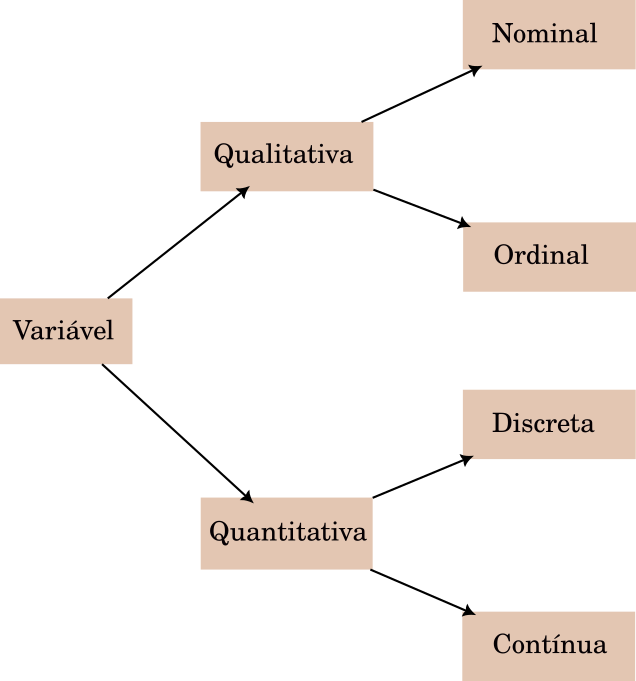
\includegraphics[width=0.5\linewidth]{figures/classificacao_variaveis.png}
    \end{figure}
\end{frame}

\begin{frame}{Tipos de variáveis}
    \textbf{Exemplo inicial }
    \begin{table}[H]
\begin{tabular}{ccccc}
\hline
Est. Civil & Instrução & Filhos & Salário & Idade \\ \hline
Solteiro          & Fundamental         & 0      & 4,00    & 26    \\
Casado          & Médio         & 1      & 4,56    & 32    \\
Casado          & Superior         & 3      & 6,20    & 34    \\
Solteiro          & Médio         & 2      & 5,23    & 21    \\
Casado          & Superior         & 2      & 3,23    & 24    \\
Solteiro          & Médio         & 1      & 7,90    & 56    \\
Casado          & Fundamental         & 4      & 6,45    & 67    \\
Casado          & Fundamental         & 0      & 4,56    & 34    \\
Solteiro          & Médio         & 1      & 6,78    & 56    \\
Solteiro          & Superior         & 0      & 3,56    & 34    \\ \hline
\end{tabular}
\end{table}
\end{frame}

\begin{frame}{Tipos de variáveis}
    \begin{atencao}
    Ao analisar as variáveis estamos olhando para a informação trazida e não para o valor em si. 
    \end{atencao}
    
    \pause
\begin{table}[H]
\begin{tabular}{ccccc}
\hline
Est. Civil & Instrução & Filhos & Salário & Idade \\ \hline
1          & 1         & 0      & 4,00    & 26    \\
2          & 2         & 1      & 4,56    & 32    \\
2          & 3         & 3      & 6,20    & 34    \\
1          & 2         & 2      & 5,23    & 21    \\
2          & 3         & 2      & 3,23    & 24    \\
1          & 2         & 1      & 7,90    & 56    \\
2          & 1         & 4      & 6,45    & 67    \\
2          & 1         & 0      & 4,56    & 34    \\
1          & 2         & 1      & 6,78    & 56    \\
1          & 3         & 0      & 3,56    & 34    \\ \hline
\end{tabular}
\end{table}
\pause
Nesse caso a tabela acima é equivalente a vista no slide anterior e a interpretação das variáveis permanece a mesma.
\end{frame}

\begin{frame}{Tipos de variáveis}
    Vamos para um exemplo real. Abrir base de dados do curso. 
\end{frame}

\begin{frame}{Tabela de frequência}
    Uma tabela de frequência relaciona categorias ou classes de valores juntamente com as frequências do número de valores que se enquadram em cada categoria ou classe. 

    Denotaremos por:
    \begin{itemize}
    \item $n_i$: Frequência absoluta
    \item $f_i$: Frequência relativa
\end{itemize}

onde, $f_i = \dfrac{n_i}{n}$
\end{frame}


\begin{frame}{Tabela de frequência}

\begin{exemplo}
    Construa a tabela de frequência para a variável formação utilizando os dados da tabela abaixo
\end{exemplo}


\begin{table}[H]
\centering
\begin{adjustbox}{width=\textwidth}
\begin{tabular}{|c|c|c|c|c|c|}
\hline
idade & experiência(anos) & sexo & cidade         & formação               & salário (R\$) \\ \hline
20    & 2                 & 1    & Rio de Janeiro & Farmácia          & 6000          \\ \hline
25    & 5                 & 0    & São Paulo      & Engenharia Química & 5000          \\ \hline
35    & 7                 & 1    & Rio de Janeiro & Farmácia          & 10000         \\ \hline
40    & 15                & 1    & Rio de Janeiro & Engenharia Química & 6000          \\ \hline
45    & 25                & 1    & Rio de Janeiro & Farmácia          & 7500          \\ \hline
22    & 1                 & 0    & São Paulo      & Farmácia          & 1740          \\ \hline
34    & 7                 & 0    & Rio de Janeiro & Farmácia          & 7000          \\ \hline
56    & 25                & 1    & São Paulo      & Engenharia Química & 6500          \\ \hline
19    & 0                 & 1    & Rio de Janeiro & Engenharia Química & 1990          \\ \hline
29    & 9                 & 0    & São Paulo      & Engenharia Química & 8000          \\ \hline
\end{tabular}
\end{adjustbox}
\end{table}

\end{frame}


\begin{frame}{Tabela de frequência}
\begin{table}[H]
\begin{tabular}{|c|c|c|}
\hline
Formação               & $n_i$  & $f_i$ \\ \hline
Farmácia          & 5      & 0,5   \\ \hline
Engenharia Química & 5      & 0,5   \\ \hline
total                  & $n$=10 & 1     \\ \hline
\end{tabular}
\end{table}
\end{frame}

\begin{frame}[fragile]
\frametitle{Tabela de frequência - Exemplo no R}
No exemplo a seguir é criado o vetor \textit{populacao} contendo 10 indivíduos, sendo armazenado o sexo (M - Masculino, F - Feminino).
\begin{block}{Tabela de frequência no R (Frequência Absoluta)}
\begin{minted}[linenos=false,breaklines]{R}
populacao = c("F", "M", "M", "F", "M", "F", "M", "F", "F", "F")
freq_absoluta = table(populacao)
print(freq_absoluta)
\end{minted}
\end{block}
\pause
Ao executar o código percebemos que a função \textit{table} retorna apenas uma tabela contendo a frequência absoluta.  
\end{frame}

\begin{frame}[fragile]
\frametitle{Tabela de frequência - Exemplo no R (Frequência Relativa)}
Uma forma de mostrar a frequência relativa é apresentada no código abaixo. 
\begin{block}{Tabela de frequência no R (Frequência Relativa)}
\begin{minted}[linenos=false,breaklines]{R}
populacao = c("F", "M", "M", "F", "M", "F", "M", "F", "F", "F")
freq_absoluta = table(populacao)
freq_relativa = prop.table(freq_absoluta)
print(freq_relativa)
\end{minted}
\end{block} 
\pause
\begin{atencao}
    Perceba que no código acima, a função que gera a tabela de frequência relativa (\textit{prop.table}) recebe como argumento a própria tabela de frequência absoluta. 
\end{atencao}

\end{frame}

\begin{frame}{Tabela de frequência - Frequência Acumulada}
    Uma coluna que pode ser últil dentro de uma tabela de frequẽncia é a coluna referente à fequência acumulada. 

    Denotaremos a frequência acumulada por $f_{ac}$, sendo obtida pela soma acumulada da coluna de frequencia relativa ($f_i$).
\end{frame}

\begin{frame}[fragile]
frametitle{Frequencia acumulada - Exemplo no R}
Para obter a frequência acumulada, basta usar a função \textit{cumsum} do R
\begin{block}{Tabela de frequência no R (Frequência Acumulada)}
\begin{minted}[linenos=false,breaklines]{R}
populacao = c("F", "M", "M", "F", "M", "F", "M", "F", "F", "F")
freq_absoluta = table(populacao)
freq_relativa = prop.table(freq_absoluta)
freq_acumulada = cumsum(freq_relativa)
\end{minted}
\end{block}   
    
\end{frame}

\begin{frame}{Tabela de frequência - Exemplo no R}
    \begin{itemize}
        \item Como gero uma tabela contendo as duas informações?
        \item Como eu gero uma tabela de frequência a partir de dados reais?
    \end{itemize}
    \begin{figure}
        \centering
        
\includegraphics[width=0.3\linewidth]{figures/turtle_doubt.png}
    \end{figure}
\end{frame}

\begin{frame}{Pausa - Aprendendo sobre DataFrames no R}
    Nome dos arquivos de código:
    
    \begin{itemize}
        \item Como criar e trabalhar com DataFrames em R: \textbf{criacao\_dataframe.R}
        \item Como criar uma tabela de frequência completa no R: \textbf{tabela\_freq.R}.
        \item Como ler bases de dados no R: \textbf{leitura\_base\_dados.R}
    \end{itemize}
    \pause
    Para aprender um pouco mais, recomendo a leitura da página 30 do livro \textbf{Uma introdução à programação com o R}.
\end{frame}
\begin{frame}
    \begin{exemplo}
        Construa uma tabela de frequência para a variável \textit{Ocupacao} da base de dados adotada no curso.
    \end{exemplo}
    
\end{frame}

\begin{frame}{Tabela de frequência com divisão em classes} 
   \begin{exemplo}
        Construa uma tabela de frequência para a variável \textit{Idade} da base de dados adotada no curso.
    \end{exemplo}
\pause
    Será que usar uma tabela de frequência é a melhor forma de apresentar esses dados?
\end{frame}

\begin{frame}{Frequência  com divisão em classes}
    A tabela de frequência  com divisão em classes é semelhante à tabela de frequência, mas com a 
    diferença que os dados são agrupados em intervalos numéricos. 
    \pause
\begin{itemize}
    \item  Geralmente a divisão em classes é bastante útil para estudar variáveis quantitativas contínuas, pois geralmente os valores não se repetem.
    \item  Tomemos como exemplo a variável salário da tabela vista anteriormente, nela apenas o valor 6000 se repete, todos os demais são únicos. Se contruísimmos uma tabela de frequência comum, a maior parte dos valores teria frequência absoluta igual a 1.
\end{itemize}
   
\end{frame}

\begin{frame}{Frequência com divisão em classes}
    \begin{exemplo}
         Em uma turma do curso de Engenharia foi feito o registro da idade de cada um dos estudantes dessa turma
        \begin{table}[G]
         \begin{tabular}{|c|c|c|c|c|c|c|c|c|c|}
            \hline
            22 & 23 & 44 & 33 & 20 & 27 & 19 & 54 & 37 & 22 \\ \hline
            25 & 29 & 40 & 23 & 20 & 30 & 24 & 39 & 28 & 21 \\ \hline
            \end{tabular}
        \end{table}

            Construa uma tabela de frequência partindo da menor idade para a variável idade. Defina a amplitude como sendo igual a 5 e inclua apenas o limite inferior dos intervalos.
    \end{exemplo}

\pause
\end{frame}

\begin{frame}{Tabela de frequência com divisão em classes} 
    \begin{table}[H]
        \begin{tabular}{cccc}
        \hline
        Idade      & $n_i$ & $f_i$ & $f_{ac}$ \\ \hline
        {[}19, 24) & 8     & 0,4   & 0,4      \\
        {[}24, 29) & 4     & 0,2   & 0,6      \\
        {[}29, 34) & 3     & 0,15  & 0,75     \\
        {[}34, 39) & 1     & 0,05  & 0,8      \\
        {[}39, 44) & 2     & 0,1   & 0,9      \\
        {[}44, 49) & 1     & 0,05  & 0,95     \\
        {[}49, 54) & 0     & 0     & 0,95     \\
        {[}54, 59) & 1     & 0,05  & 1        \\
        total      & n=20  &   1    &          \\ \hline
        \end{tabular}
        \end{table}
\end{frame}

\begin{frame}{Tabela de frequência  com divisão em classes} 
\begin{itemize}
    \item Como determinar a \textbf{amplitude dos intervalos}?
    \pause
    \item Todos os intervalos devem possuir a mesma amplitude?
    \pause
    \item Devemos usar intervalos abertos, semi-abertos ou fechados?
\end{itemize}
\end{frame}

\begin{frame}[fragile]
\frametitle{Tabela de frequência com divisão em classes - Exemplo no R}

No exemplo a seguir, iremos construir uma tabela de frequência com divisão em classes para a variável idade,
definindo a amplitude como sendo igual a 5 e incluindo apenas o limite inferior dos intervalos.

\begin{block}{Tabela de frequência  com divisão em classes no R (Amplitudes Iguais)}
\begin{minted}[linenos=false,breaklines]{R}
require("readxl")
dados = read_excel(file.choose(), sheet=1) 
idades = dados$Idade
tabela_freq = table(cut(idades, seq(min(idades), max(idades), 5)))
\end{minted}
\end{block}
\end{frame}

\begin{frame}[fragile]
\frametitle{Tabela de frequência  com divisão em classes - Exemplo no R}
    No exemplo do slide anterior, utilizamos a função \textit{cut} passando como segundo argumento uma sequência. 
    Podemos também passar como argumento o número de intervalos, dessa forma a própria função define a amplitude. 
\begin{block}{Tabela de frequência com divisão em classes no R (Amplitudes Iguais)}
\begin{minted}[linenos=false,breaklines]{R}
require("readxl")
dados = read_excel(file.choose(), sheet=1) 
idades = dados$Idade
tabela_freq = table(cut(idades, 6))
\end{minted}
\end{block}
Note que ao rodar o código acima temos 6 intervalos, não necessariamente de mesma amplitude. 
\end{frame}


\begin{frame}{Gráficos - Gráfico de dispersão}
    O gráfico de dispersão permite representar dados de duas ou três variáveis. Consiste em basicamente em dispor cada ponto no planno cartesiano. 
    \begin{figure}
    \centering
    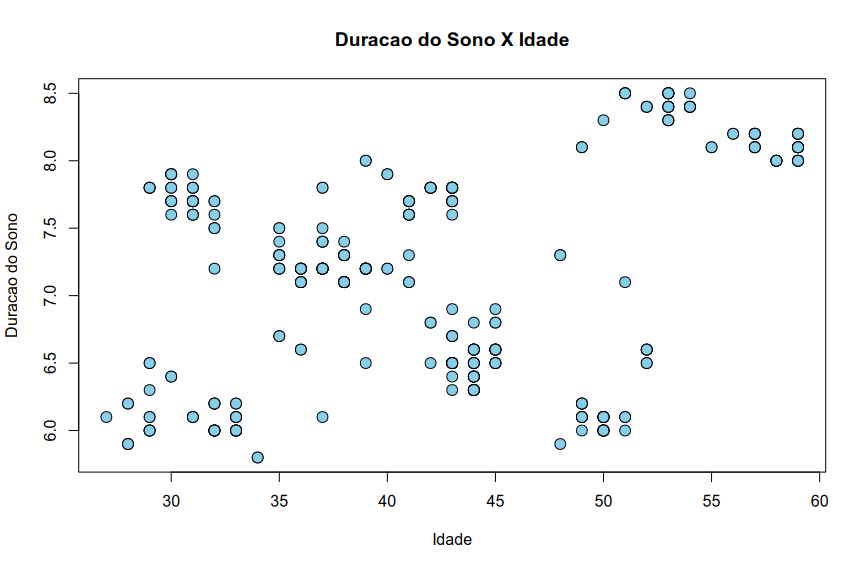
\includegraphics[width=0.8\linewidth]{figures/grafico_dispersao.png}
    \end{figure}
\end{frame}

\begin{frame}{Interpretação - Gráfico de dispersão}
    Em geral, a interpretação de um gráfico de dispersão se concentra em avaliar o comportamento de uma variável em relação à outra. 

    Na Figura do slide anterior, podemos observar que \textbf{parece} que ao aumentar a idade, também há o aumento da duração do sono. 
\end{frame}

\begin{frame}[fragile]
    \frametitle{Gráficos - Gráfico de dispersão - Exemplo no R }
    
\begin{block}{Gráfico de dispersão no R}
\begin{minted}[linenos=false,breaklines]{R}
require("readxl")
dados = read_excel(file.choose(), sheet=1) 
duracao_sono = dados$`Duracao do Sono`
idade = dados$Idade
plot(x=idade, y=duracao_sono,
     main="Duracao do Sono X Idade",
     xlab ="Idade", ylab = "Duracao do Sono",
     bg = "#87ceeb", # Cor dos pontos
     cex = 1.5, # Tamanho dos pontos
     pch=21) # Tipo do ponto      
\end{minted}
    \end{block}
    \end{frame}

\begin{frame}{Gráficos - Gráfico de setores (pizza)}
    Consiste em dividir um círculo (pizza) em diferentes setores (fatias),
     cada um representando a proporção do elemento analisado em relação ao conjunto de estudo. 
    \begin{figure}
        \centering
        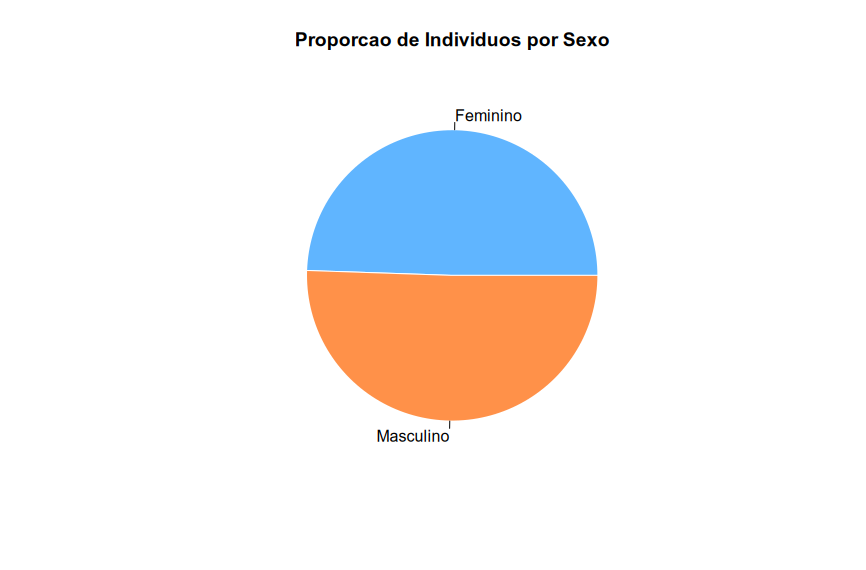
\includegraphics[width=0.8\linewidth]{figures/grafico_pizza.png}
    \end{figure}
\end{frame}

\begin{frame}
    \begin{atencao}
        Olhando para o gráfico do slide anterior, qual sexo parece ter maior proporção?
    \end{atencao}
    

    \pause

    Devido a esse problema, recomenda-se evitar o uso de gráficos de pizza. Sendo recomendado:

    \begin{itemize}
        \item Colocar as porcentagens por extenso caso existam poucas categorias.
        \item Usar outro gráfico, como por exempo o gráfico de barras. 
    \end{itemize}
\end{frame}

\begin{frame}[fragile]
    \frametitle{Gráficos - Gráfico de setores (pizza) - Exemplo no R}
    
    \begin{block}{Gráfico de pizza no R}
    \begin{minted}[linenos=false,breaklines]{R}
require("readxl")
dados = read_excel(file.choose(), sheet=1) 
sexo = dados$Sexo
freq_sexo = table(sexo)
pie(freq_sexo,
    border="white", # Coloca bordas brancas
    col=c("#60B5FF", "#FF9149"), # Cor de cada fatia
    main = "Proporcao de Individuos por Sexo")
\end{minted}
\end{block}
\end{frame}

\begin{frame}{Gráficos - Gráfico de barras}
\begin{itemize}
    \item Utiliza o plano cartesiano com os valores da variável no eixo das abcissas e as frequências ou porcentagens no eixo das ordenadas. 
    \pause
    \item Utilizado, geralmente, para representar visualmente uma tabela de frequência.
\end{itemize}

\pause
\begin{figure}
    \centering
    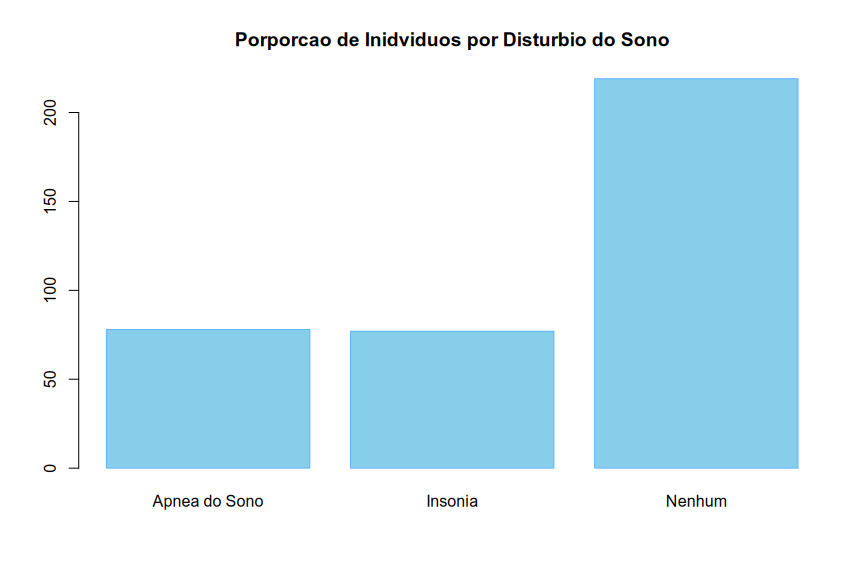
\includegraphics[width=0.8\linewidth]{figures/grafico_barras.png}
    \caption{Gráfico de barras para a variável cidade}
\end{figure}
\end{frame}

\begin{frame}{Interpretação - Gráfico de barras}

    \begin{itemize}
        \item No gráfico de barras, estamos interessados em entender a altura da barra referente a cada categoria analisada. 
        \pause
        \item Na Figura do slide anterior, podemos perceber que \textbf{parece} que temos a mesma proporção de indivíduos com apnea do sono e insonia, sendo 
        o fato de não ter nenhum disturbio a Característica maoritariamente presente no conjunto de dados. 
    \end{itemize}
\end{frame}


\begin{frame}[fragile]
\frametitle{Gráficos - Gráfico de barras - Exemplo no R}
\begin{block}{Gráfico de barras no R}
\begin{minted}[linenos=false,breaklines]{R}
require("readxl")
dados = read_excel(file.choose(), sheet=1) 
disturbio_sono = dados$`Disturbio do Sono`
freq_disturbio = table(disturbio_sono)
barplot(freq_disturbio, 
        main="Porporcao de Inidviduos por Disturbio do Sono",
        border="#60B5FF",# Cor do contorno das barras
        col="#87ceeb") # Cor das barras
\end{minted}
\end{block}
\end{frame}

\begin{frame}{Gráficos - Histograma}
    \begin{itemize}
        \item  O histograma é bastante semelhante ao gráfico de barras.
        \pause
        \item  Utilizado, em geral, como uma uma representação visual da uma tabela agrupada em classes. 
        \pause
        \item Evidencia a distribuição de uma variável quantitativa. 
    \end{itemize}
\pause

\begin{figure}
    \centering
    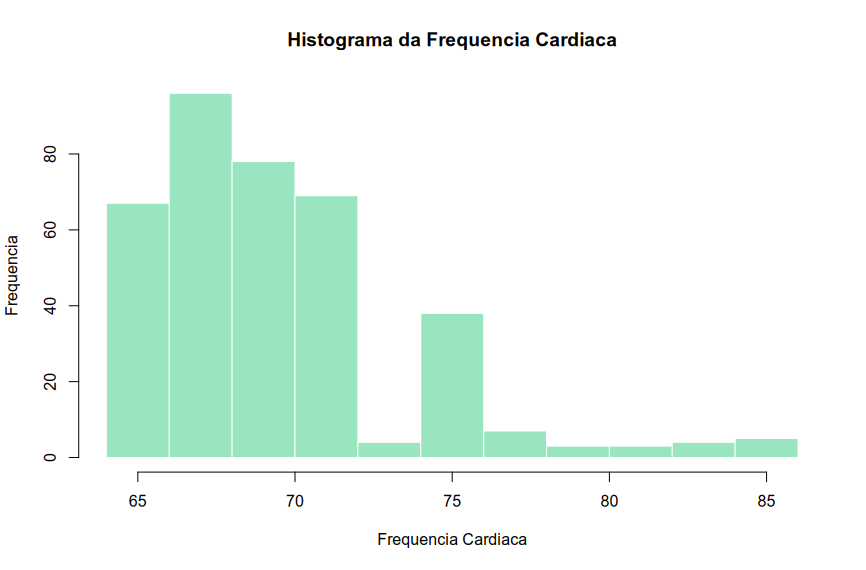
\includegraphics[width=0.8\linewidth]{figures/grafico_histograma.png}
\end{figure}
\end{frame}

\begin{frame}{Interpretação - Histograma}
    \begin{itemize}
        \item  Ao olhar para um histograma estamos interessados em analisar a distribuição dos valores, tentando
        perceber a concentração dos valores para a variável analisada.
        \pause
        \item Uma outra possibilidade é tentar identificar algum padrão, podendo relacionar com distribuições estatísticas conhecidas. 
        \item Na Figura do slide anterior, poodemos perceber que há uma maior concentração de frequências cardiacas antes do valor 72 batimentos por minuto.  
    \end{itemize}

\end{frame}

\begin{frame}[fragile]
\frametitle{Gráficos - Histograma - Exemplo no R}
\begin{block}{Histograma no R}
\begin{minted}[linenos=false,breaklines]{R}
require("readxl")
dados = read_excel(file.choose(), sheet=1) 
freq_cardiaca = dados$`Frequencia Cardiaca`
hist(freq_cardiaca, 
     main="Histograma da Frequencia Cardiaca",
     xlab = "Frequencia Cardiaca",
     ylab = "Frequencia",
     breaks=8, # Numero de barras (Nem sempre)
     col="#33CC8080", # Cor das barras
     border=FALSE) # Elimina as bordas
\end{minted}
\end{block}
\end{frame}

\begin{frame}{Gráficos - Histograma}
    \begin{itemize}
        \item O argumento breaks define o número de barras, entretanto, para esse gráfico, todas as barras devem ter o mesmo tamanho. 
        \pause
        \item Também é possível passar uma tabela de frequencia em classes dentro da função. 
    \end{itemize}
\end{frame}

\begin{frame}{Gráficos - Boxplot}
    De forma inicial, o gráfico Boxplot apresenta a distribuição dos dados, mas, diferentemente do histograma, apresenta alguns elementos específicos, os quais
    serão vistos posteriormente. 

    \pause

    \begin{figure}
        \centering
        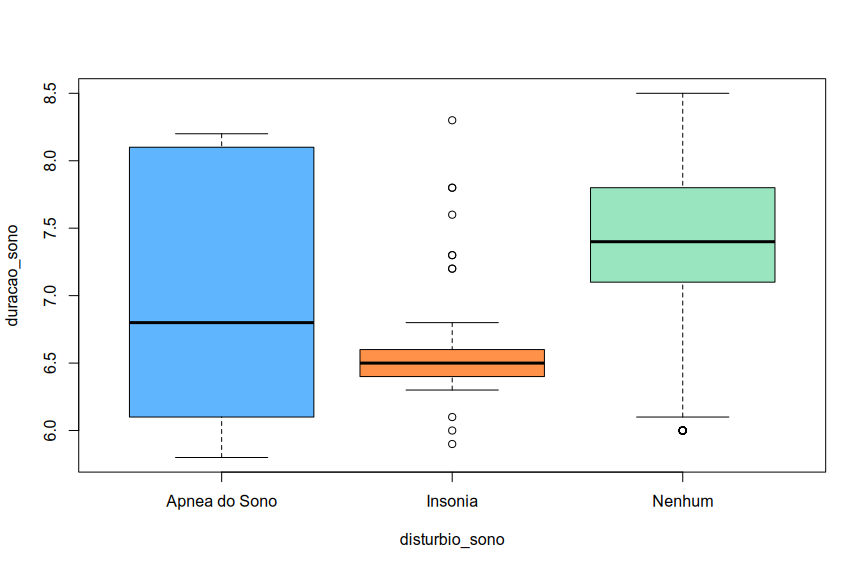
\includegraphics[width=0.8\linewidth]{figures/grafico_boxplot.png}
    \end{figure}
\end{frame}

\begin{frame}[fragile]
\frametitle{Gráficos - Extras}
\begin{block}{Gráfico de uma função matemática}
\begin{minted}[linenos=false,breaklines]{R}
modulo = function(x){
    return(abs(x))
}
curve(modulo,
    -2, 2, # Intervalo do eixo x
    ylim=c(0, 3), # Intervalo do eixo y
    col="#60B5FF", # Cor do grafico
    ann=FALSE) # Remove nomes nos eixos
\end{minted}
\end{block}
\end{frame}

\begin{frame}[fragile]
\frametitle{Gráficos - Extras}
\begin{block}{Adicionar linhas verticais e horizontais}
\begin{minted}[linenos=false,breaklines]{R}
modulo = function(x){
    return(abs(x))
}
curve(modulo, -2, 2, ylim=c(0, 3),
      col="#60B5FF",
      ann=FALSE) 
abline(h=0) # Adiciona uma linha horizontal y=0
abline(v=0) # Adiciona uma linha vertical x=0
\end{minted}
\end{block}
\end{frame}


\begin{frame}[fragile]
    \frametitle{Gráficos - Extras}
    \begin{block}{Vários Gráficos em uma mesma Imagem}
    \begin{minted}[linenos=false,breaklines]{R}
modulo = function(x){
    return(abs(x))
}
quadratica = function(x){
    return(x^2)
}
curve(modulo, -2, 2, col="#60B5FF",
      ann=FALSE, ylim=c(0, 3))
par(new=TRUE)
curve(quadratica, -2, 2, col="#FF9149",
      axes=FALSE, ann=FALSE, ylim=c(0, 3))
\end{minted}
\end{block}
\end{frame}

\begin{frame}[fragile]
\frametitle{Gráficos - Extras}
\begin{block}{Adicionando pontos no plano cartesiano}
\begin{minted}[linenos=false,breaklines]{R}
modulo = function(x){
    return(abs(x))
}
quadratica = function(x){
    return(x^2)
}
curve(modulo, -2, 2, col="#60B5FF",
      ann=FALSE, ylim=c(0, 3))
par(new=TRUE)
curve(quadratica, -2, 2, col="#FF9149",
      axes=FALSE, ann=FALSE, ylim=c(0, 3))
points(-1, 1, col='red', pch=19) # Adiciona um ponto vermelho no ponto (-1,1)
points(1, 1, col='red', pch=19)  # Adiciona um ponto vermelho no ponto (1,1)      
\end{minted}
\end{block}
\end{frame}

\begin{frame}{Gráficos - Exemplos a não serem seguidos}
    \begin{figure}
        \centering
        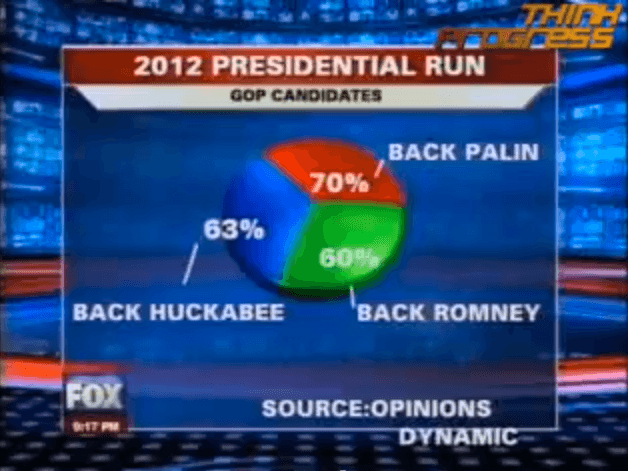
\includegraphics[width=0.8\linewidth]{figures/lie_1.png}
    \end{figure}
\end{frame}

\begin{frame}{Gráficos - Exemplos a não serem seguidos}
    \begin{figure}
        \centering
        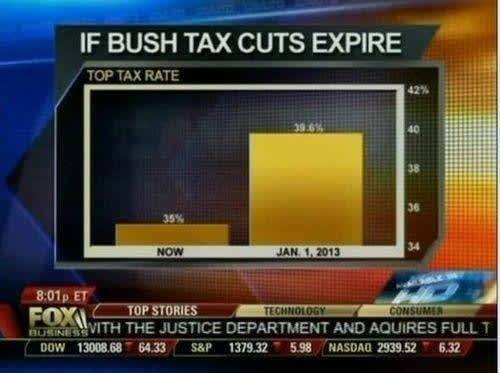
\includegraphics[width=0.8\linewidth]{figures/lie_2.jpeg}
    \end{figure}
\end{frame}


\begin{frame}{Gráficos - Exemplos a não serem seguidos}
    \begin{figure}
        \centering
        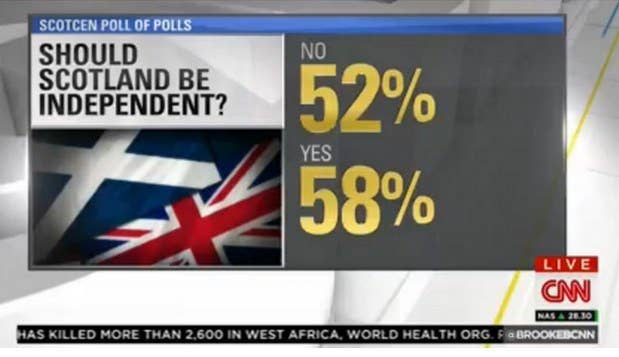
\includegraphics[width=0.8\linewidth]{figures/lie_4.jpg}
    \end{figure}
\end{frame}

\begin{frame}{Gráficos - Exemplos a não serem seguidos}
    \begin{figure}
        \centering
        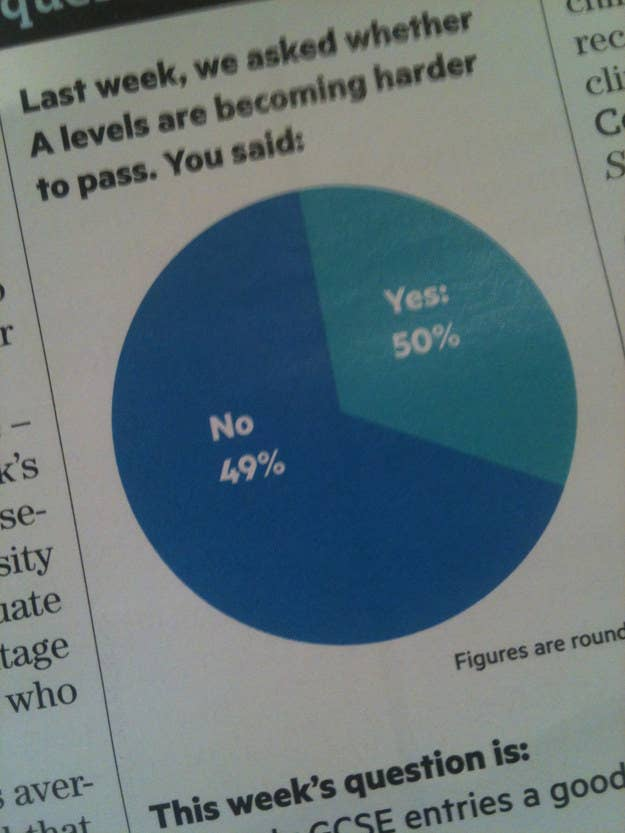
\includegraphics[width=0.5\linewidth]{figures/lie_5.jpg}
    \end{figure}
\end{frame}

\begin{frame}{Gráficos - Exemplos a não serem seguidos}
    \begin{figure}
        \centering
        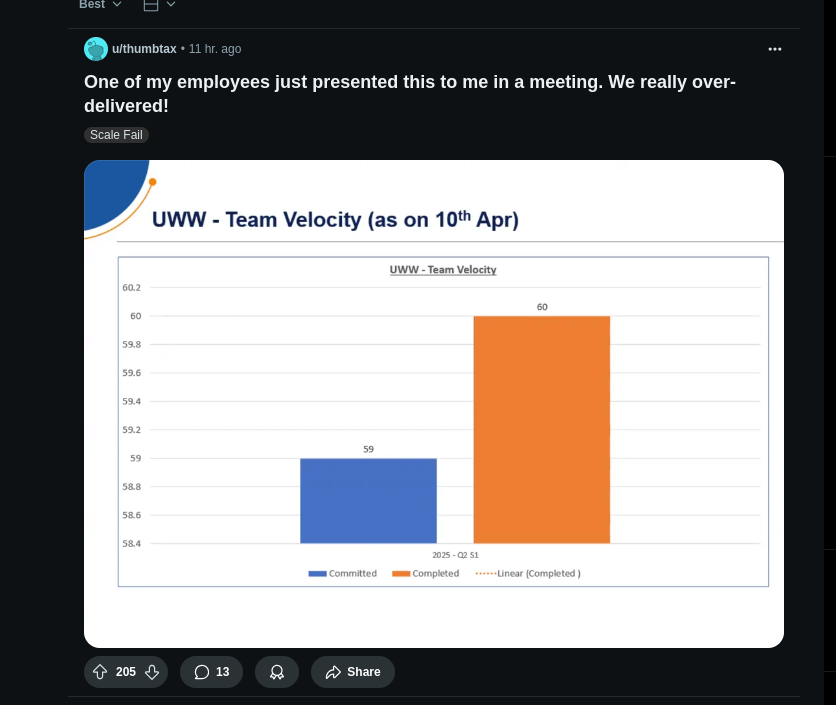
\includegraphics[width=0.8\linewidth]{figures/lie_6.png}
    \end{figure}
\end{frame}


\begin{frame}{Gráficos - Exemplos a não serem seguidos}
    \begin{figure}
        \centering
        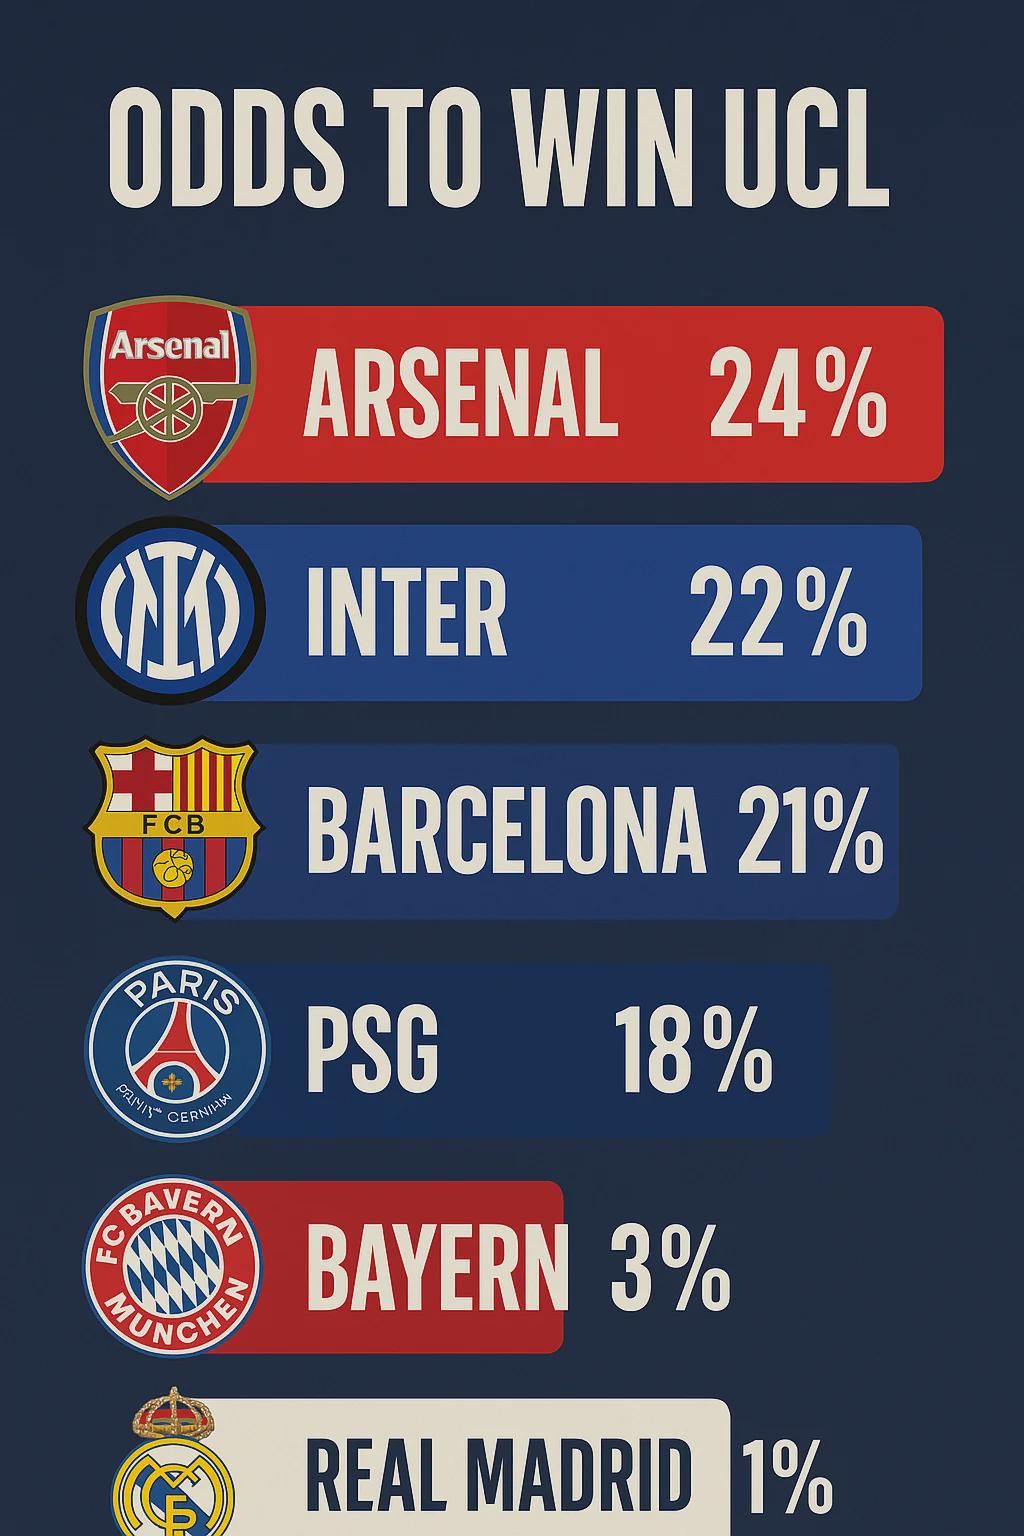
\includegraphics[width=0.4\linewidth]{figures/lie_7.jpeg}
    \end{figure}
\end{frame}

\begin{frame}{Medidas de Posição}

Podemos ter o interesse em resumir nosso conjunto de dados, apresentando um ou mais valores que de certa forma representem todo o conjunto de dados.

Para determinar esses valores, utiliza-se as \textbf{medidas de posição central}: Média, Mediana e Moda. 

\end{frame}

\begin{frame}{Média Aritmética}

Dado um conjunto de $n$ observações $x_1, x_2, \dots, x_n$ a média aritmética é definida como:

$$\Bar{x} = \dfrac{\sum\limits_{i=1}^n x_i}{n} = \dfrac{x_1 + \dots + x_n}{n}$$

\end{frame}

\begin{frame}{Média Aritmética}
\begin{exemplo}
    Suponha que tenhamos coletado a altura de $10$ alunos de uma turma, as alturas obtidas foram as seguintes:
    $$1,90; 1,67; 1,87; 1,55; 1,76; 1,87; 1,95; 1,66; 1,75; 1,60$$
\end{exemplo}

Logo, 

{\footnotesize $$\Bar{x} = \dfrac{1,90 + 1,67 + 1,87 + 1,55 + 1,76 + 1,87 + 1,95 + 1,66 + 1,75 + 1,60}{10} = 1,76$$}
\end{frame}

\begin{frame}[fragile]
\frametitle{Média Aritmética - Exemplo no R}    
Para calcular a média de um conjunto de dados no R, utilizamos a função \textit{mean}.
\begin{block}{Calculando a Média Aritmética no R}
\begin{minted}[linenos=false,breaklines]{R}
altura =  c(1.90, 1.67, 1.87, 1.55, 1.76, 1.87, 1.95, 1.66, 1.75, 1.60)
media_altura = mean(altura)
\end{minted}
\end{block}
\end{frame}

\begin{frame}{Média Aritmética}
\begin{exemplo}
    Obtenha a média da Idade dos indivíduos do conjunto de dados adotado na disciplina.
\end{exemplo}    
\end{frame}

\begin{frame}{Moda}
    A moda de um conjunto de dados, representada por $x^*$, é o valor que mais se repete, 
    ou seja, o valor mais frequente. 
    \pause

    \begin{atencao}
        Um conjunto de dados pode ter mais de uma moda.
    \end{atencao}
\end{frame}

\begin{frame}{Mediana}

Seja $x_1, x_2, \dots, x_n$ um conjunto de $n$ observações, e seja $x_{(i)}, i=1, \dots, n$
o conjunto das observações ordenadas, de modo que $x_{(1)} \leq x_{(2)} \leq \dots \leq x_{(n)}$.
Então, a mediana $Q_2$ é definida como o valor tal que 50\% das observações são menores
e 50\% são maiores que ela. 
\pause
\begin{exemplo}   

Suponhamos que o peso de 7 crianças de uma determinada turma escolar tenha sido coletada, os pesos coletados são exibidos a seguir:

$$28, 34, 45, 39, 42, 33, 50$$

Obtenha a mediana desse conjunto de dados
\end{exemplo}
\end{frame}

\begin{frame}{Mediana}
Primeiramente vamos ordenar os dados:

$$28, 33, 34, 39, 42, 45,  50$$

\pause 
Logo, a mediana será o valor $39$

\end{frame}

\begin{frame}{Mediana}
\begin{exemplo}
Retomemos o exemplo das alturas dos alunos, temos os seguintes dados:

$$1,90; 1,67; 1,87; 1,55; 1,76; 1,87; 1,95; 1,66; 1,75; 1,60$$

\end{exemplo}

Para calcular a mediana, primeiramente vamos ordenar os dados:

$$ 1,55; 1,60; 1,66; 1,67; 1,75; 1,76;  1,87;  1,87; 1,90; 1,95$$

\pause

Temos 10 elementos, logo, não conseguimos encontrar o valor que divide exatamente ao meio o conjunto de dados, nesse caso, a mediana é dada pela média dos elementos que ocupam a posição $\frac{n}{2}$ e $\frac{n}{2} +1 $.

$$Q_2 = \dfrac{1,75 + 1,76}{2} = 1,755$$
\end{frame}

\begin{frame}{Mediana}
Portanto, 
$$Q_2 = \begin{cases}
    x_{\left(\frac{n+1}{2} \right)} & \text{se n é impar}\\
    \dfrac{x_{\left(\frac{n}{2}\right)} + x_{\left(\frac{n}{2} + 1 \right)} }{2} & \text{se n é par}\\
\end{cases}$$
\end{frame}

\begin{frame}[fragile]
\frametitle{Médiana - Exemplo no R}   
Para obter a mediana de um conjunto de dados no R, basta usar a função \textit{median}
\begin{block}{Calculando a Mediana no R}
\begin{minted}[linenos=false,breaklines]{R}
require("readxl")
dados = read_excel(file.choose(), sheet=1) 
idades = dados$Idade
mediana_idade = median(idades)
\end{minted}
\end{block}
\end{frame}

\begin{frame}{Média X Mediana}

\begin{itemize}
    \item Imagine que você precisa atravessar um lago e existe uma placa que diz: Altura média do lago: $1,5$ metros. Você o atravessaria?
    \pause
    \item Dependendo do conjunto de dados, nem sempre a média é uma boa medido da resumo. A média é fortemente influenciada por valores aberrantes (outliers). 
\end{itemize}

\pause

\begin{exemplo}
    Os seguintes dados referentes aos salários (em R\$) de cinco funcionários de uma firma: $$136; 210; 350; 360; 2500$$ Calcule o salario médio. 
\end{exemplo}

\end{frame}

\begin{frame}{Média X Mediana}
    No caso do slide anterior, o salário médio é igual a $R\$ 647,20$. No entanto, esse valor não representa, de forma adequada, os salários mais
    baixos e os salários mais altos, isso porque o mais alto é muito diferente dos demais.
     
\end{frame}

\begin{frame}{Média X Mediana}
    \begin{itemize}
        \item Por outro lado, a mediana desse conjunto de dados é o valor $350$, que indica que metade dos valores é menor que $350$ e a outra metade maior. 
        \item Ainda assim, não conseguimos capturar o quanto menor ou maior são. 
    \end{itemize}
\end{frame}

\begin{frame}{Observações}
\begin{itemize}
    \item Quando a média é próxima a mediana dizemos que isso é um indicativo de que a amostra não apresenta pontos aberrantes (possíveis outliers).
    \item A média é fortemente influenciada pela presença de pontos aberrantes, enquanto a mediana não é.
\end{itemize}
    
\end{frame}

\begin{frame}{Média Ponderada}
    A média aritmética ponderada de números $x_1, x_2, \dots, x_n$ com pesos
    $w_1, w_2, \dots, w_n$ é definida como:

    $$\bar{x}_w = \dfrac{w_1x_1 + w_2x_2 + \dots + w_nx_n }{w_1 +w_2 + \dots + w_n} = \dfrac{\sum_{i=1}^n w_i x_i}{\sum_{i=1}^n w_i}$$
\end{frame}

\begin{frame}{Quartis - Elementos fundamentais}
    \begin{itemize}
        \item O primeiro quartil, que indicaremos por $Q_1$, deixa 25\% das observações abaixo e 75\% acima dele. 
        \pause
        \item A mediana é o segundo quartil
        \pause
        \item O terceiro quartil, $Q_3$, deixa 75\% das observações abaixo e 25\% acima dele. 
    \end{itemize}
    
\end{frame}

\begin{frame}{Quartis - Elementos adicionais}
    \begin{itemize}
        \item Amplitude Interquartil (AIQ) = $Q_3 - Q_1$
        \pause
        \item Limite Superior = $Q_3 + 1,5 \cdot AI$
        \pause
        \item Limite Inferior = $Q_1 - 1,5 \cdot AI$
    \end{itemize}
   
\end{frame}

\begin{frame}{Quartis - Cálculo dos quartis}
    $$Q_1 = x_{\left(\frac{1}{4}(n+1) \right)}$$
    \pause
    $$Q_3 =  x_{\left(\frac{3}{4}(n+1)\right)} $$
    \textcolor{red}{Importante:} Se o valor obtido não for um inteiro, fazer uma média do elemento que ocupa a parte inteira e seu sucessor.
\end{frame}

\begin{frame}[fragile]
\frametitle{Quartis - Exemplo no R}   
Para obter os quartis de um conjunto de dados no R, utilizamos a função \textit{quantile}.
\begin{block}{Variância no R}
\begin{minted}[linenos=false,breaklines]{R}
require("readxl")
dados = read_excel(file.choose(), sheet=1) 
duracao_sono = dados$`Duracao do Sono`
q1 = quantile(duracao_sono, 0.25) # Primeiro quartil
q3 = quantile(duracao_sono, 0.75) # Terceiro quartil
\end{minted}
\end{block}
\end{frame}

\begin{frame}{Revisitando o Boxplot}
    \begin{figure}
    \centering
    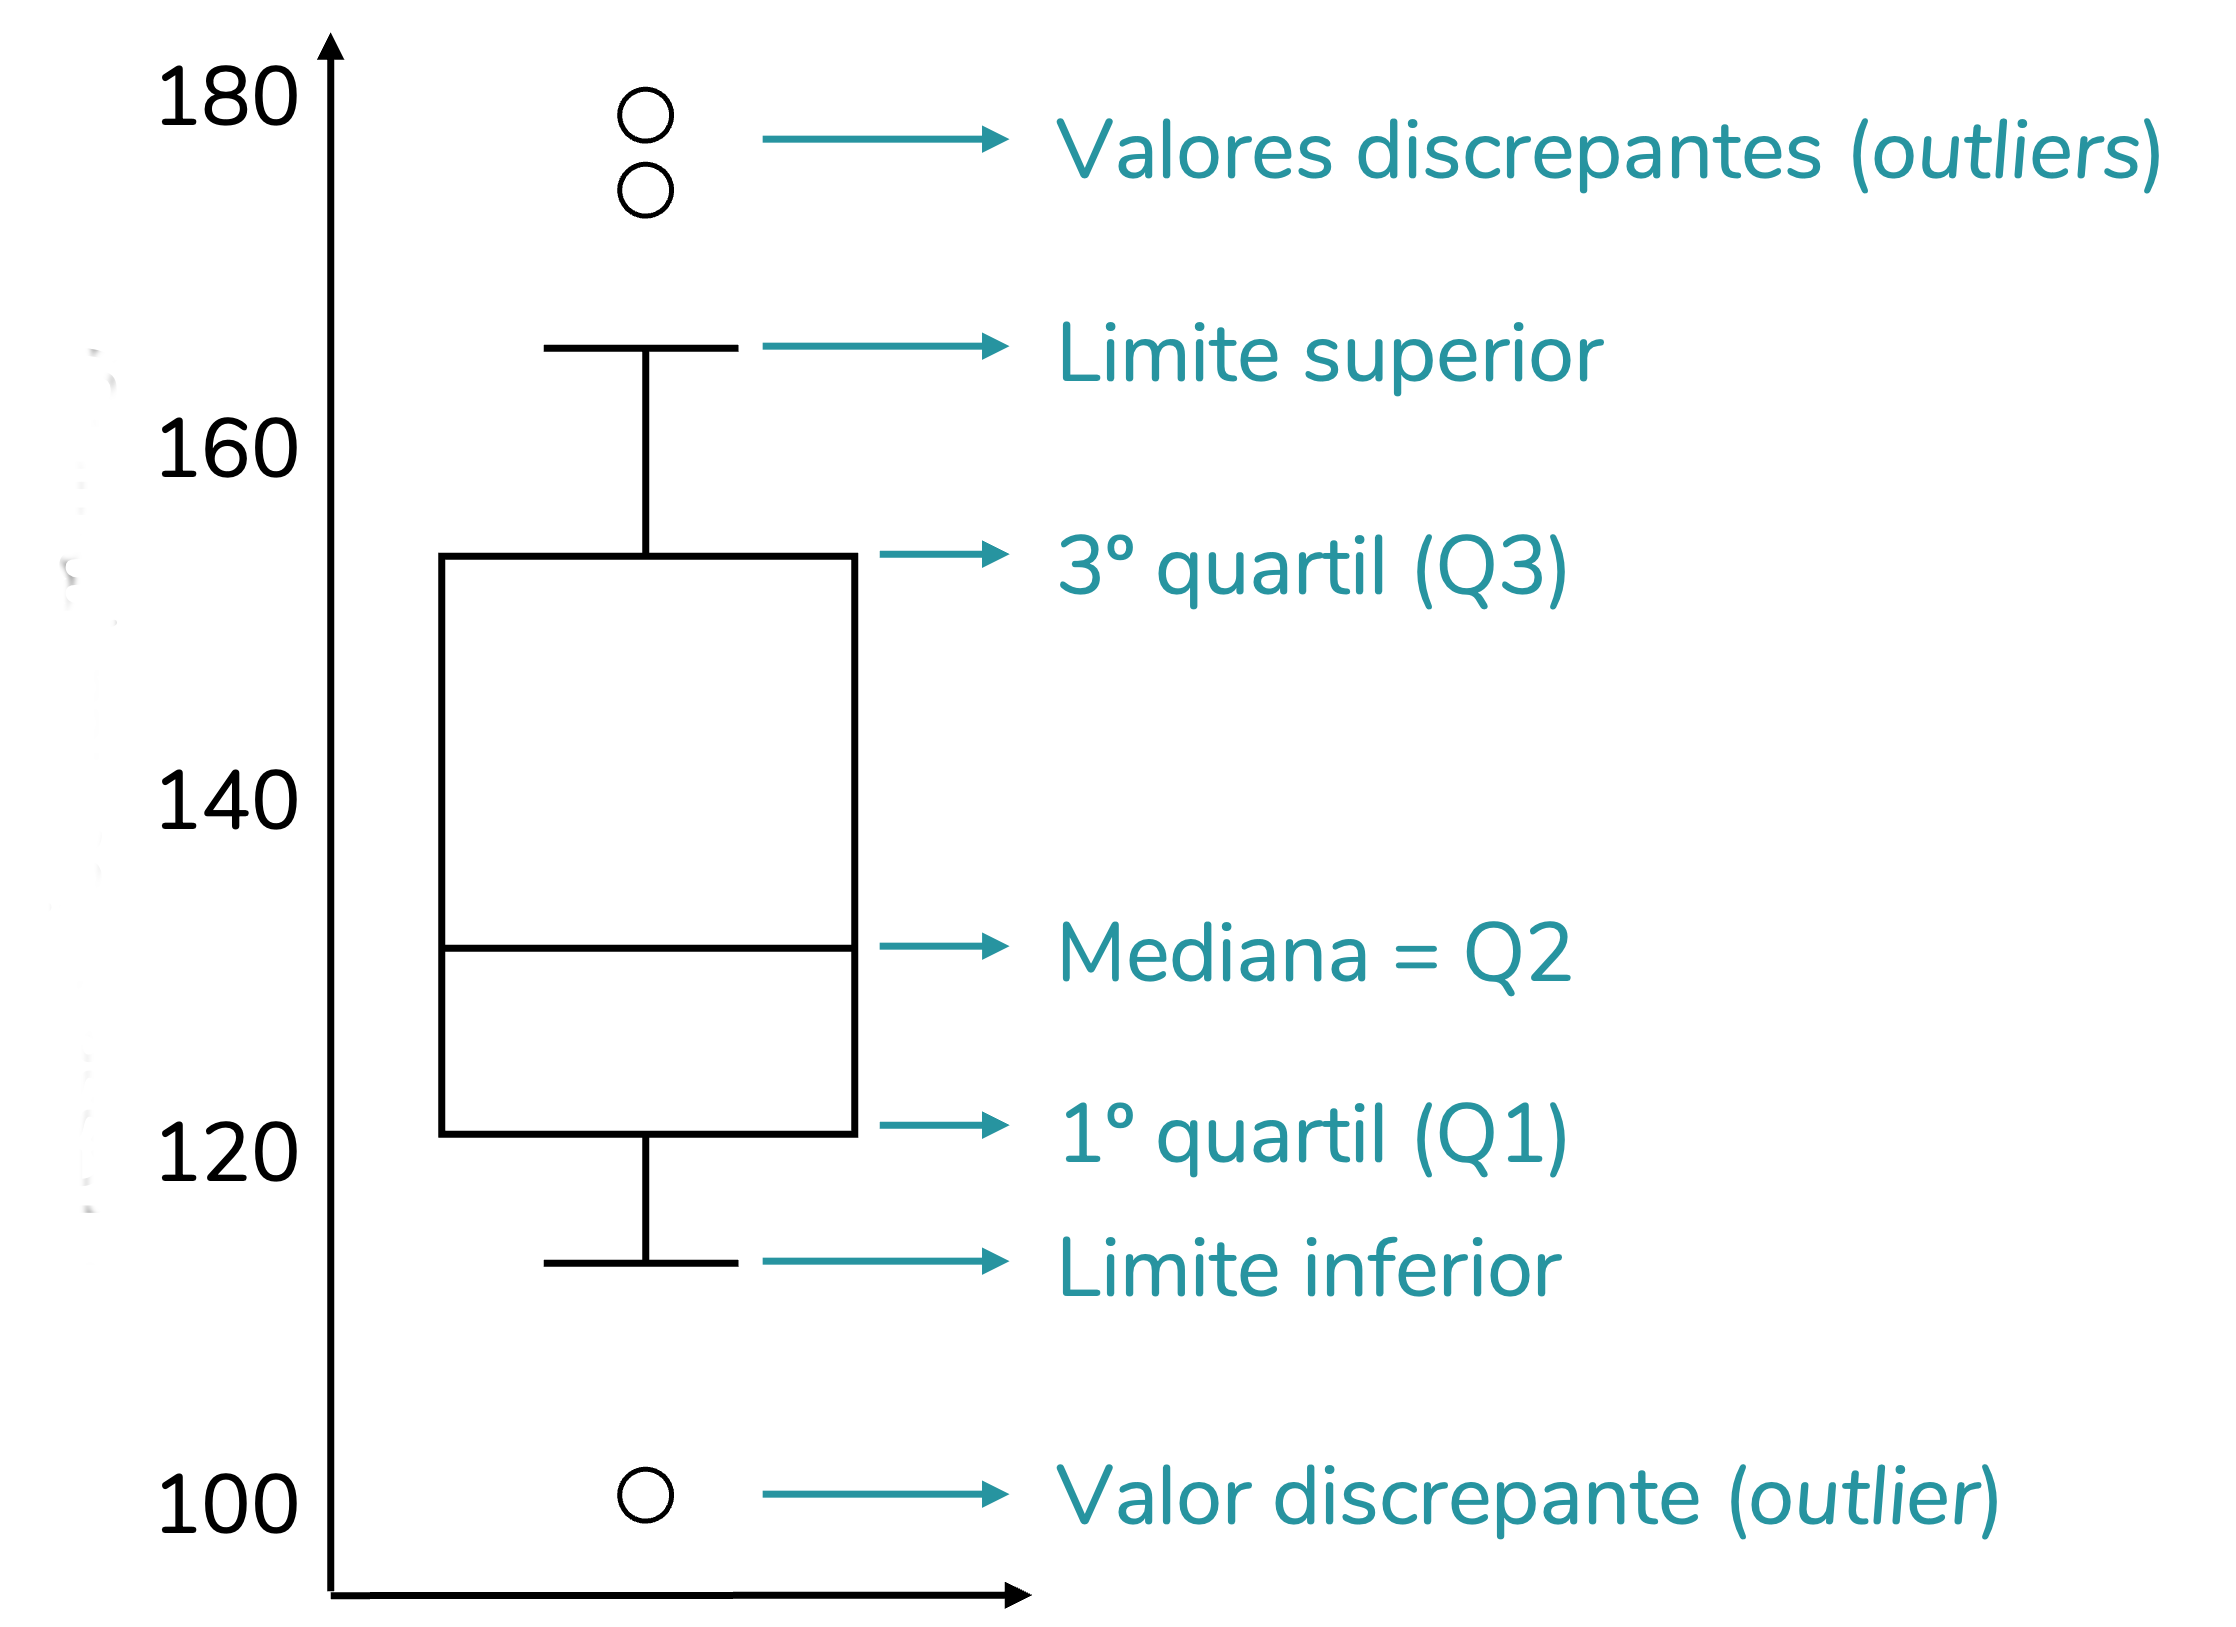
\includegraphics[width=0.6\linewidth]{figures/boxplot.png}    
    \end{figure}
\end{frame}

\begin{frame}[fragile]
\frametitle{Boxplot - Exemplo no R}   
\begin{block}{Gráfico Boxplot no R}
\begin{minted}[linenos=false,breaklines]{R}
require("readxl")
dados = read_excel(file.choose(), sheet=1) 
disturbio_sono = dados$`Disturbio do Sono`
duracao_sono = dados$`Duracao do Sono`
boxplot(duracao_sono ~ disturbio_sono,
        col=c("#60B5FF", "#FF9149", "#33CC8080"))
\end{minted}
\end{block}
\end{frame}
\begin{frame}{Medidas de dispersão}

Muitas vezes estamos interessados em entender o comportamento dos dados e as medidas de posição não são suficientes:

\begin{exemplo}
    Calcule a média dos seguintes conjuntos de dados:
    $$salarios_1 = 2.000,00 ; 3.500,00 ; 4.900,00 ; 3.100,00 $$
    $$salarios_2 = 3.375,00 ; .3375,00; 3.375,00; 3.375,00$$
\end{exemplo}
\end{frame}

\begin{frame}{Medidas de dispersão}
    \begin{exemplo}
        Calcule a mediana dos seguintes conjuntos de dados:
        $$salarios_1 = 2.000,00 ; 3.500,00 ; 4.900,00 ; 3.100,00; 4.100,00 $$
        $$salarios_2 = 2.000,00 ; 3.500,00 ; 70.900,00 ; 3.100,00; 32.000,00 $$
    \end{exemplo}
\end{frame}

\begin{frame}
Em ambos os casos anteriores, percebemos que a Média e Mediana não são suficientes para descrever o comportamento dos dados. Devido a isso, 
trabalharemos agora com medidas de dispersão, sendo elas: Amplitude, Devio médio absoluto, Variância, Desvio Padrão e Coeficiente de Variação.
\end{frame}


\begin{frame}{Amplitude}
    A amplitude de um conjunto de dados é a distância entre o maior valor e o menor valor.
    \pause
    $$\Delta_{total} = V_{max} - V_{min}$$
    \pause
    A amplitude nos dá uma ideia do intervalo de possíveis valores que a variável analisada pode assumir. 
\end{frame}

\begin{frame}[fragile]
\frametitle{Amplitude - Exemplo no R}   
Para calcular a amplitude de um conjunto de dados no R, utilizamos a função \textit{var}.
\begin{block}{Amplitude no R}
\begin{minted}[linenos=false,breaklines]{R}
require("readxl")
dados = read_excel(file.choose(), sheet=1) 
duracao_sono = dados$`Duracao do Sono`
amplitude_duracao_sono = max(duracao_sono) - min(duracao_sono)
\end{minted}
\end{block}
\end{frame}

\begin{frame}{Desvio médio absoluto}

 O desvio médio absoluto de um conjunto de dados $x_1, x_2, \dots, x_n$ é definido por:
$$DMA(X) = \dfrac{\sum\limits_{i=1}^n |x_i - \Bar{x}|}{n}$$

\pause 
\begin{itemize}
    \item O desvio médio tem como objetivo verificar quanto os valores, em média, estão se distanciando da média.
    \pause
    \item Note que o desvio médio absoluto é sempre um valor positivo. 
\end{itemize}
\pause
\begin{exemplo}
    Calcule o desvio médio para os salários dos exemplos anteriores. 
\end{exemplo}    

\end{frame}

\begin{frame}{Variância}
    A variância $\sigma^2$ de um conjunto de dados $x_1, x_2, \dots, x_n$ é definida por 
    $$\sigma^2 = \dfrac{\sum\limits_{i=1}^n (x_i - \Bar{x})^2}{n}$$
\pause
\begin{itemize}
    \item Perceba que a variância é bastante semelhante ao desvio médio absoluto, no entanto, penaliza grandes desvios. 
    \pause
    \item Observe que a variância é sempre um número \textbf{positivo}.
    \pause
    \item Note que a variância \textbf{não} fornece um valor na mesma unidade de medida dos dados. 
    \pause
    \item A variância não tem interpretação prática direta, podendo ser utilizada como comparação. 
\end{itemize}
\end{frame}

\begin{frame}{Variância}
\begin{exemplo}
    Calcule a variância para os salários dos exemplos anteriores. 
\end{exemplo}    
\end{frame}

\begin{frame}[fragile]
    \frametitle{Variância - Exemplo no R}   
    Para calcular a variância de um conjunto de dados no R, utilizamos a função \textit{var}.
    \begin{block}{Variância no R}
    \begin{minted}[linenos=false,breaklines]{R}
    require("readxl")
    dados = read_excel(file.choose(), sheet=1) 
    duracao_sono = dados$`Duracao do Sono`
    var_duracao_sono = var(duracao_sono)
    \end{minted}
    \end{block}
\end{frame}

\begin{frame}{Desvio padrão}

O desvio padrão de um conjunto de dados $x_1, x_2, \dots, x_n$ é definido como a raiz 
quadrada da variância:
\pause
$$\sigma =\sqrt{\sigma^2}$$
\pause

\begin{itemize}
    \item Diferentemente da variância, o desvio padrão possui interpretação prática, pois ele volta o valor para a unidade de medida dos dados.
    \pause
    \item Interpretamos o desvio padrão como quanto, em média, os valores do conjunto de dados estão se ditanciando da média. 
    \pause
    \item Note que, apesar de interpretável, é difícil dizer se temos um desvio padrão alto ou baixo, mas, com o auxilio da amplitude, podemos tirar boas conclusões. 
\end{itemize}
\end{frame}

\begin{frame}{Coeficiente de variação}
Dado um conjunto de observações $x_1, x_2, \dots, x_n$; o coeficiente de variação
(CV) é definido como a razão entre o desvio-padrão dos dados e sua média,
ou seja,

 $$CV = \dfrac{\sigma}{\Bar{x}}$$

 \begin{itemize}
    \item Em geral, multiplica-se o valor do CV por 100 para ter um valor percentual. 
    \pause
    \item Quanto menor for o valor do CV, mais homogêneo é um conjunto de dados.
 \end{itemize}
\end{frame}

\begin{frame}{Coeficiente de variação}
    Podemos adotar o seguinte critério:
    \begin{itemize}
        \item $CV < 0,10 \implies$ variabilidade baixa 
        \item $0,10 \leq CV < 0,20 \implies$ variabilidade intermediária
        \item $0,20 \leq CV < 0,30 \implies$ variabilidade alta
        \item $CV \geq 0,30 \implies$ variabilidade muito alta
    \end{itemize}

    \textbf{Observação: Só podemos calcular o CV quando a média amostral for diferente de zero.}
\end{frame}

\begin{frame}{Escores padronizados}
    Suponhamos que tenha sido feito um estudo visando entender o desempenho dos alunos do curso de Engenharia Química no curso de Cálculo em comparação com o curso de Estatística. 
    \pause
    \vspace{5px}
    
    As notas de 9 alunos da turma foram coletadas e são apresentadas abaixo:

    \centering
    \begin{tabular}{lccccccccc}
    \toprule
    Aluno & 1 & 2 & 3 & 4 & 5 & 6 & 7 & 8 & 9 \\
    \midrule
    Estatística & 6 & 4 & 5 & 7 & 8 & 5 & 5 & 5 & 7 \\
    Cálculo     & 6 & 8 & 9 & 10 & 7 & 7 & 8 & 9 & 3 \\
    \bottomrule
    \end{tabular}

    Olhando para as notas, será que tirar 6 em Estatística tem o mesmo "peso" que tirar 6 em Cálculo?
\end{frame}

\begin{frame}{Escores Padronizados}
    \centering
    \begin{tabular}{lccccccccc}
    \toprule
    Aluno & 1 & 2 & 3 & 4 & 5 & 6 & 7 & 8 & 9 \\
    \midrule
    Estatística & 6 & 4 & 5 & 7 & 8 & 5 & 5 & 5 & 7 \\
    Cálculo     & 6 & 8 & 9 & 10 & 7 & 7 & 8 & 9 & 3 \\
    \bottomrule
    \end{tabular}

    Vamos calcular a média das notas de cada um dos cursos:
    $$\bar{x}_{E} = \dfrac{6 + 4 + 5 + 7 + 8 + 5 + 5 + 5 + 7}{9} = \dfrac{52}{9} = 5,78$$
    \pause
    $$\bar{x}_{C} = \dfrac{6 + 8 + 9 + 10 + 7 + 7 + 8 + 9 + 3}{9} = \dfrac{67}{9} = 7,44$$

    \pause
    \begin{itemize}
        \item Podemos perceber que, o aluno 1, por exemplo, ficou acima da média em Estatística, mas abaixo da média em Cálculo.
        \pause
        \item Outra forma de verificar essa afirmação é por meio do \textbf{desvio}.
    \end{itemize}
\end{frame}

\begin{frame}{Escores Padronizados - Desvio}
    O desvio de uma observação $x_i$ em torna da média é definido como:

    $$d_i = x_i - \bar{x}$$

    \pause

    Calculando os desvios da nota do primeiro aluno, temos:

    $$d_{E_1} = 6 - 5,78 = 0,22$$
    $$d_{C_1} = 6 - 7,44 = -1,44$$

    \pause

    \begin{itemize}
        \item Dessa forma, temos que o aluno 1 ficou, aproximadamente, $0,22$ pontos acima da média em Cálculo e 1,44 abaixo da média em Estatística.  
        \pause
        \item Ainda asssim, não temos como comparar se o desempenho do aluno foi melhor em Estatística ou em Cálculo, pois, novamente, as médias são diferentes. 
    \end{itemize}
\end{frame}

\begin{frame}{Escores Padronizados}
    \centering
    \begin{tabular}{lccccccccc}
    \toprule
    Aluno & 1 & 2 & 3 & 4 & 5 & 6 & 7 & 8 & 9 \\
    \midrule
    Estatística & 6 & 4 & 5 & 7 & 8 & 5 & 5 & 5 & 7 \\
    Cálculo     & 6 & 8 & 9 & 10 & 7 & 7 & 8 & 9 & 3 \\
    \bottomrule
    \end{tabular}

    Vamos calcular o desvio padrão das notas de cada um dos cursos. 

    $$\sigma^2_{E} = 1,51 \implies \sigma_{E} = 1,23$$
    \pause
    $$\sigma^2_{C} = 3,80 \implies \sigma_{C} = 1,95$$

    \pause
    \begin{itemize}
        \item Qual disciplina apresenta maior variabilidade das notas?
        \pause
        \item Faça o cálculo da variância manualmente e verifique os resultados apresentados nesse slide. 
    \end{itemize}
\end{frame}

\begin{frame}{Escores Padronizados}

    O escore padronizado de uma observação $x_i$ é definido como:

    $$z_i = \dfrac{x_i - \bar{x}}{\sigma_x}$$

    \pause

    \begin{itemize}
        \item Ao dividirmos pelo desvio padrão, a escala passa a ser definida em termos do desvio padrão e cada escore padronizado nos informa que a observação está 
        acima ou abaixo da média por um determinado número de desvios-padrão. Dessa forma, removemos o efeito das médias e o fato das variabilidades serem diferentes. 
        \item \textcolor{red}{Importante}: A média dos escores padronizados é, independente do conjunto de dados, sempre igual a $0$ e a variância igual a $1$.
    \end{itemize}
\end{frame}

    \begin{frame}{Escores Padronizados}
     Vamos analisar agora as notas de Estatística e Cálculo em termos dos escores padronizados:

     \centering
     \resizebox{\textwidth}{!}{%
     \begin{tabular}{llccccccccc}
     \toprule
     \multicolumn{2}{c}{Aluno} & 1 & 2 & 3 & 4 & 5 & 6 & 7 & 8 & 9 \\
     \midrule
     \multirow{2}{*}{Estatística} & Nota   & 6 & 4 & 5 & 7 & 8 & 5 & 5 & 5 & 7 \\
                                  & Escore & 0{,}18 & -1{,}45 & -0{,}63 & 1{,}00 & 1{,}81 & -0{,}63 & -0{,}63 & -0{,}63 & 1{,}00 \\
     \midrule
     \multirow{2}{*}{Cálculo}     & Nota   & 6 & 8 & 9 & 10 & 7 & 7 & 8 & 9 & 3 \\
                                  & Escore & -0{,}74 & 0{,}29 & 0{,}80 & 1{,}13 & -0{,}23 & -0{,}20 & 0{,}29 & 0{,}80 & -3{,}28 \\
     \bottomrule
     \end{tabular}
     }
    
    \begin{itemize}
        \item Podemos perceber que a nota 6 está, aproximadamente, $0,18$ desvios-padrão acima da média em Estatística
         e aproximadamente $0,74$ desvios-padrão abaixo da média das notas de Cálculo. 
         \item Perceba que tirar a nota 10 em Cálculo é menos "surpreendente" que tirar 8 em Estatística.  
    \end{itemize}
\end{frame}

\begin{frame}{Escores Padronizados - Teorema de Chebyshev}
    Para qualquer distribuição de dados, pelo menos $(1 - 1/z^2)$ dos dados estão dentro de $z$ desvios-padrão da média, onde $z$ é qualquer valor maior que 1. 
    Ou seja, pelo menos (1-1/z^2) dos dados estão no intervalo $\[\bar{x} - z\sigma; \bar{x} + z\sigma\]$.

\end{frame}

\begin{frame}{Escores Padronizados - Teorema de Chebyshev}
    Exemplos:
    \begin{itemize}
        \item Para $z=2$ temos que $1-1/z^2 = 3/4 = 75\%$ dos dados estão dentro de dois desvios-padrão da média. Ou, equivalentemente, 
        75\% dos escores padronizados estão no intervalo $(-2,2)$. 
        \pause
        \item Para $z=3$  que $1-1/z^2 = 8/9 = 89\%$ dos dados estão dentro de três desvios-padrão da média. Ou, equivalentemente, 
        89\% dos escores padronizados estão no intervalo $(-3,3)$. 
        \pause
        \item Para $z=4$  que $1-1/z^2 = 15/16 = 93,75\%$ dos dados estão dentro de quatro desvios-padrão da média. Ou, equivalentemente, 
        93,75\% dos escores padronizados estão no intervalo $(-4,4)$. 
    \end{itemize}
\end{frame}

\begin{frame}{Covariância e Correlação}
    \begin{itemize}
        \item  Até agora, vimos como analisar medidas referentes a uma única variável. Entretanto, na prática, 
        podemos nos deparar com situaçãos nas quais se faz interessante estudar a relação entre duas ou mais
        variáveis. 
        \pause
        \item    Nesse sentido, surge a Covariância e a Correlação, que são medidas usadas para analisar a relação entre duas ou mais variáveis.  
    \end{itemize}
\end{frame}

\begin{frame}{Covariância}
    A covariância entre duas variáveis $X$ e $Y$ é definida por:

    $$Cov(X,Y) = \dfrac{\sum_{i=1}^n (x_i - \bar{x})(y_i - \bar{y}) }{n}$$

    \pause

    \begin{itemize}
        \item A covariância mede o grau de associação \textbf{linear} entre as variáveis.
        \pause
        \item A unidade de medida é dada pelo produto das unidades de medida das variáveis X e Y.
        \pause
        \item  \textcolor{red}{Importante}: A covariância depende da escala dos dados, o que faz com que seja difícil estabelecer comparações. 
        \pause
        \item  Seus valores podem variar de $-\infty$ a $\infty$
    \end{itemize}
\end{frame}


\begin{frame}[fragile]
    \frametitle{Covariância - Exemplo no R}   
    Para calcular a covariãncia entre duas variáveis no R, utilizamos a função \textit{cov}.
    \begin{block}{Covariância no R}
    \begin{minted}[linenos=false,breaklines]{R}
    dados = read.csv(file.choose())
    duracao_sono = dados$`Duracao do Sono`
    idade = dados$Idade
    cov_dsono_idade = cov(duracao_sono, idade)
    \end{minted}
    \end{block}
\end{frame}

\begin{frame}{Impacto da escala dos dados no cálculo da covariância}
    \begin{itemize}
        Exemplo no R, arquivo: escala\_covariancia.R 
    \end{itemize}
\end{frame}

\begin{frame}{Coeficiente de correlação}
    O coeficiente de correlação entre duas variáveis $X$ e $Y$ é definido por:

    $$Corr(X,Y) = \rho(X,Y) = \dfrac{1}{n} \sum_{i=1}^n \left( \dfrac{x_i - \bar{x}}{\sigma_X}\right) \left( \dfrac{y_i - \bar{y}}{\sigma_Y}\right)$$

    \pause
    \begin{itemize}
        \item O coeficiente de correlação também mede o grau de associação \textbf{linear} entre as variáveis.
        \pause
        \item  O coeficiente de correlação \textbf{não} depende da escala dos dados, permitindo comparações. 
        \pause
        \item Seus valores podem variar entre $-1$ e $1$.
    \end{itemize}
\end{frame}

\begin{frame}{Classificação do coeficiente de correlação}
    
\begin{table}[H]
\centering
\begin{tabular}{|c|l|}
\hline
\textbf{Valor de $\rho$ (+ ou –)} & \textbf{Interpretação} \\ \hline
0{,}00 a 0{,}19 &  Correlação bem fraca \\ \hline
0{,}20 a 0{,}39 &  Correlação fraca \\ \hline
0{,}40 a 0{,}69 &  Correlação moderada \\ \hline
0{,}70 a 0{,}89 &  Correlação forte \\ \hline
0{,}90 a 1{,}00 &  Correlação muito forte \\ \hline
\end{tabular}
\end{table}
\end{frame}

\begin{frame}[fragile]
\frametitle{Correlação - Exemplo no R}   
    Para calcular o coeficiente de correlação entre duas variáveis no R, utilizamos a função \textit{cor}.
    \begin{block}{Correlação no R}
    \begin{minted}[linenos=false,breaklines]{R}
    dados = read.csv(file.choose())
    duracao_sono = dados$`Duracao do Sono`
    idade = dados$idade
    cor_dsono_idade = cor(duracao_sono, idade)
    \end{minted}
    \end{block}
\end{frame}

\begin{frame}{Correlação \textbf{Linear} ( Apenas Linear)}
    Exemplo no R, arquivo: correlacao\_linear.R
\end{frame}

\begin{frame}{Correlação não implica causalidade}
    \begin{figure}
        \centering
        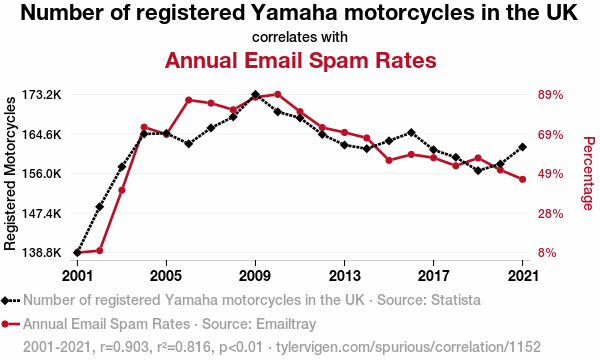
\includegraphics[width=0.8\linewidth]{figures/1152_number-of-registered-yamaha-motorcycles-in-the-uk_correlates-with_annual-email-spam-rates.png}
    \end{figure}
\end{frame}


\begin{frame}{Correlação não implica causalidade}
    \begin{figure}
        \centering
        
\includegraphics[width=0.8\linewidth]{figures/2011_masters-degrees-awarded-in-engineering-technologies_correlates-with_hydopower-energy-generated-in-vietnam.png}
    \end{figure}
\end{frame}


\begin{frame}{Correlação não implica causalidade}
    \begin{figure}
        \centering
        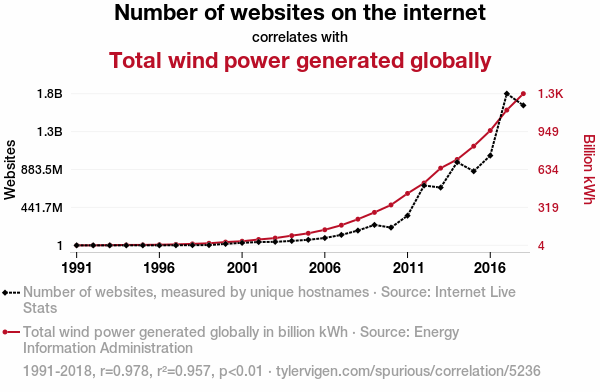
\includegraphics[width=0.8\linewidth]{figures/5236_number-of-websites-on-the-internet_correlates-with_total-wind-power-generated-globally.png}
    \end{figure}
\end{frame}

\begin{frame}{Fim!}
    Chegamos ao fim da primeira parte da matéria de estatística! 

    \pause

    \vspace{5px}

    Antes de passarmos para a Probabilidade, vamos falar sobre os seguintes pontos:

    \begin{itemize}
        \item Como usar o Quarto. 
        \item Lacunas do R (salvar DataFrame, filtrar DataFrame, valores únicos e obter dimensões do dataframe )
        \item Explicação do trabalho. 
    \end{itemize}
\end{frame}
